\documentclass[twoside,a4paper]{article}
\usepackage{geometry}
\geometry{margin=1.5cm, vmargin={0pt,1cm}}
\setlength{\topmargin}{-1cm}
\setlength{\paperheight}{29.7cm}
\setlength{\textheight}{25.3cm}

% useful packages.
\usepackage{amsfonts}
\usepackage{amsmath}
\usepackage{amssymb}
\usepackage{amsthm}
\usepackage{enumerate}
\usepackage{graphicx}
\usepackage{multicol}
\usepackage{fancyhdr}
\usepackage{layout}

% some common command
\newcommand{\dif}{\mathrm{d}}
\newcommand{\avg}[1]{\left\langle #1 \right\rangle}
\newcommand{\difFrac}[2]{\frac{\dif #1}{\dif #2}}
\newcommand{\pdfFrac}[2]{\frac{\partial #1}{\partial #2}}
\newcommand{\OFL}{\mathrm{OFL}}
\newcommand{\UFL}{\mathrm{UFL}}
\newcommand{\fl}{\mathrm{fl}}
\newcommand{\op}{\odot}
\newcommand{\Eabs}{E_{\mathrm{abs}}}
\newcommand{\Erel}{E_{\mathrm{rel}}}

\begin{document}

\pagestyle{fancy}
\fancyhead{}
\lhead{NAME Jiatu Yan}
\chead{Numerical Analysis homework \#4}
\rhead{Date 2020.4.12}


\section*{I. The max-norm of errors for intervals number n}
\begin{tabular}{|c|c|}
\hline
n&max-norm of error\\
\hline
5&0.350000000000000\\
\hline
10&0.100052988118413\\
\hline
20&0.052883146381976\\
\hline
40&0.023491579385279\\
\hline
80&0.007228575231679\\
\hline
\end{tabular}

We can find that the errors is in inverse proportion to the index of the number of intervals.

\section*{II \small{Plot the interpolating splines.}}

\begin{figure}[h]
	\centering
	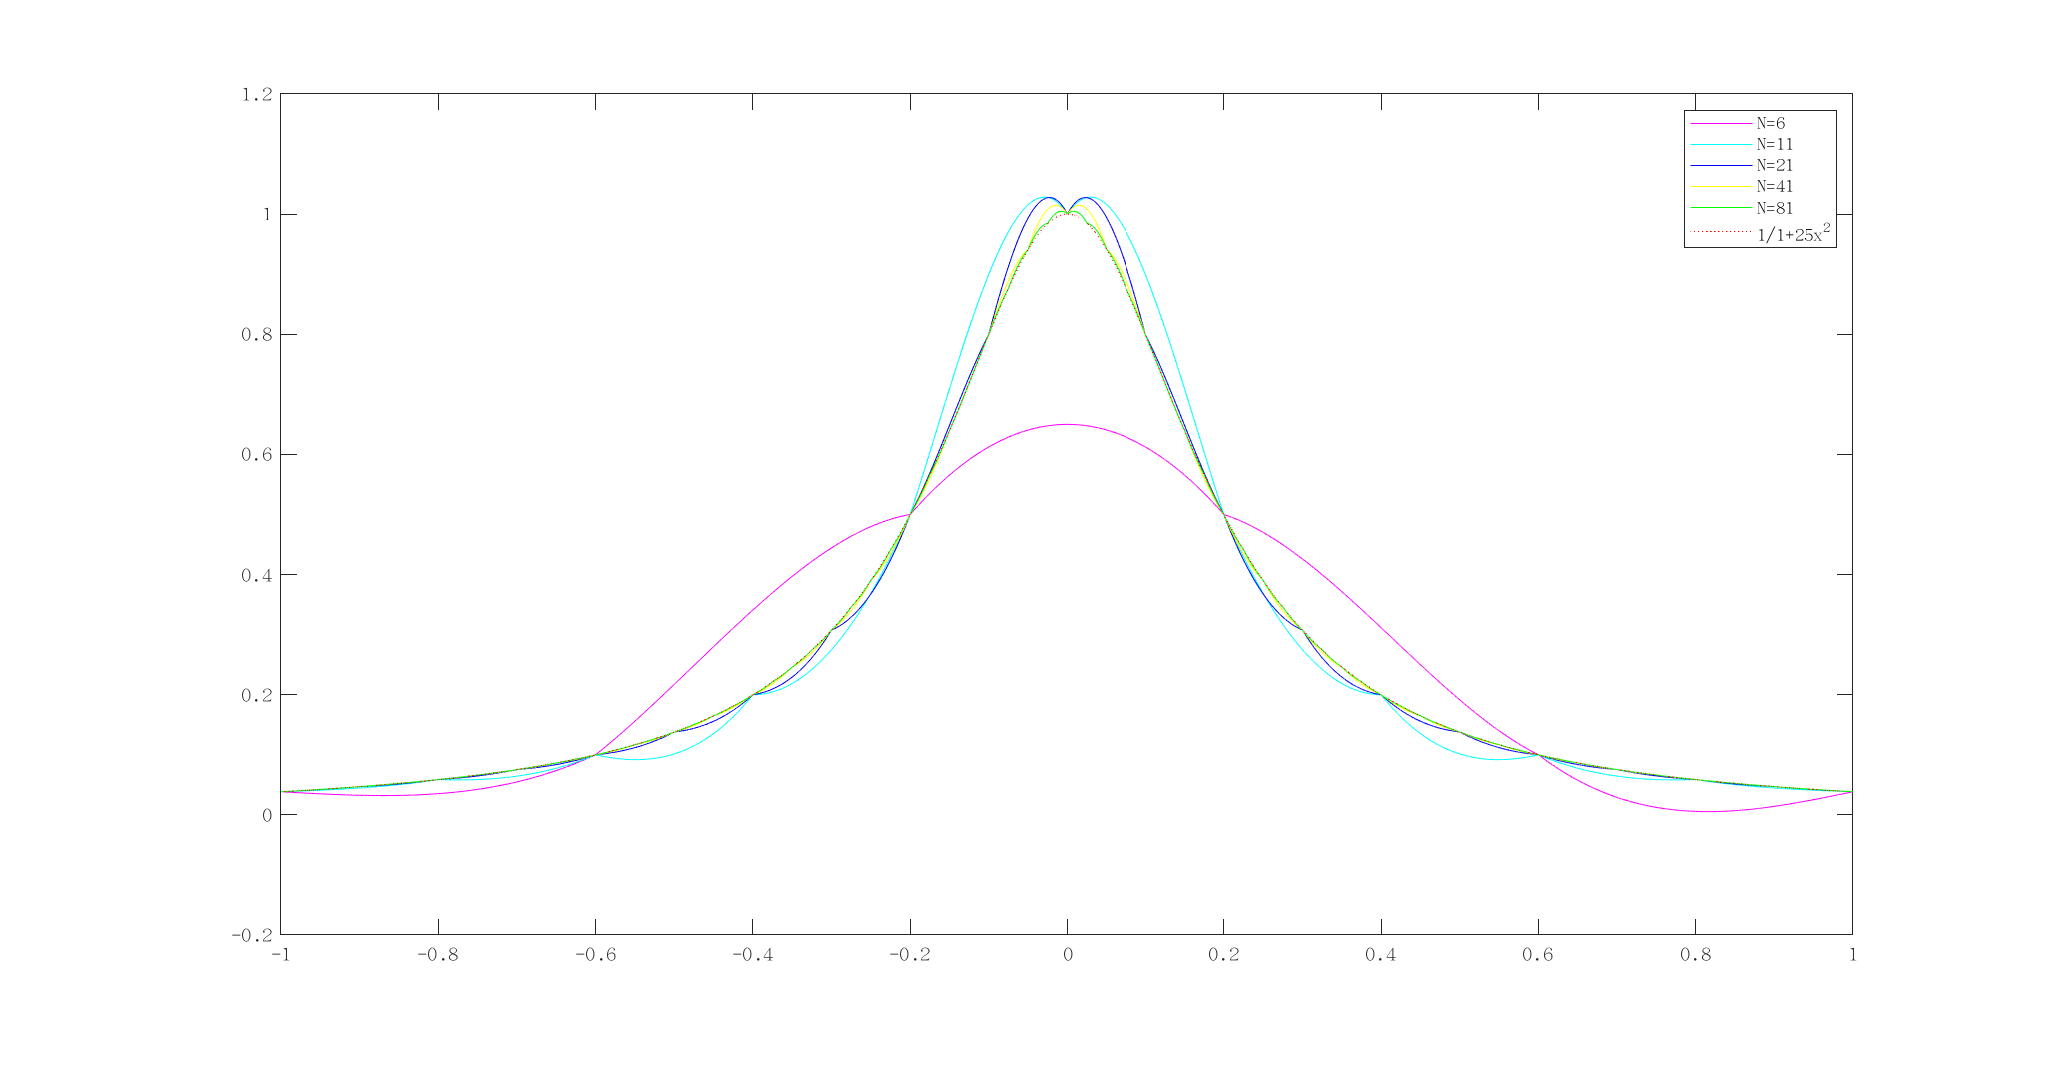
\includegraphics[width=10cm, height=5cm]{Plot.eps}
	\caption{The interpolating splines.}
\end{figure}

We can find that spline interpolation is free of the wide oscillations in the Runge phenomenon.

\end{document}

%%% Local Variables: 
%%% mode: latex
%%% TeX-master: t
%%% End: 
